\documentclass{amsart}
\usepackage{graphicx}

\newsavebox{\covmat}% Box to store covariancematrix content
\savebox{\covmat}{$\left(\begin{smallmatrix}1+(m+1)^2&m(m+1)+1\\m(m+1)+1&1+m^2\end{smallmatrix}\right)$}
\newsavebox{\intmat}
\savebox{\intmat}{$\left(\begin{smallmatrix}1&-1\\-m&m+1\end{smallmatrix}\right)$}

\begin{document}

We want to build a circuit that performs an analog modulus operation. Our reasoning for why we want to build such a circuit is explained below. \\

%We'd like to communicate information across a limited-bandwidth channel. 
We'd like to represent a waveform with a fixed number of bits per second.
Our waveform is composed of data points generated from a set of possibly-correlated sources. In our analysis of the method in the paper, we assume that the waveforms are drawn from a Gaussian distribution, but this is just to simplify the analysis. In fact, the data in the waveforms could be drawn from any distribution we choose, and could be related to other data in the waveforms in any way we choose. \\

We would like to represent these data points as cheaply as possible, while minimally disturbing the information they contain. \\

Let us momentarily ignore the fact that there are multiple sources of information that are correlated to each other. If we would like to represent the information contained only in a single data point drawn from a Gaussian distribution, the naive approach is already clearly suboptimal. If the Gaussian was centered about 0 with variance 1, and we observed the value 0.573, it would be wasteful to send the floating-point number directly over the channel. First, it's not clear how many bits we should allocate to ourselves; if we want to be safe and allow ourselves a huge number of bits, most of those bits will be going towards communicating very little information (in most cases, they'll be telling us that the value is between -1 and 1). Importantly, we will be failing to take into account the fact that the Gaussian has a lot more probability density in the center than at the edges; we'd be using the same number of bits to communicate that the value was between 3 and 4 (very unlikely to happen) as we would be to communicate that the value was between 0 and 1 (reasonably likely to happen). \\

By taking the modulus of the value that we observe, we can send only the low-order bits, which are the bits that we're unsure about anyhow, and the receiver can simply guess that the value we sent was the likeliest value for us to have sent. In the example above, we might take the value we observed modulo 2; if we sent 0.573 over the channel, the receiver would guess that we were likelier to have observed 0.573 instead of 2.573 or -1.427, and will interpret our message as ``0.573'' as a result. At the moment, we aren't doing anything different from committing to sending only values within a certain range correctly. \\

However, the situation becomes more interesting when we send multiple correlated values over the channel. The values we send over the channel reveal information about each other, so even after a very small modulus is taken, we can infer a lot of information about which ``bins'' each of the data points fell into (by ``bin'' I mean whether the value was between -1 and 1, or -3 and -1, or 1 and 3, if we'd chosen 2 as our bin size). \\

Naturally, the most accurate way to make use of the information given by the correlations is to consider the likelihood of every possible mapping of values to bins. To give a concrete example, let us suppose that in addition to generating and sending 0.573, we also generated a second data point drawn from the same distribution, which took on a value of -0.821. Let us suppose also that the sender and the receiver both understand that the two data points are strongly correlated. After we sent both values over the channel, the most accurate way for the receiver to decide what the true values were would be to consider each possible mapping of values to bins. The receiver might conclude that there's a good chance that the first value was 0.573 and that the second value was 1.179 ($1.179 \equiv -0.821$ modulo 2). The receiver might also conclude that there was a good chance that the first value was -1.427 and that the second value was  -0.821. The receiver would probably conclude there was a less good chance that the values were 0.573 and -0.821 or, even less likely, -1.427 and 1.179, because of the strong correlation between the two values. Put simply, the receiver would try to choose a pair of values that was both close together, and that was near the center of the distribution, since that's where most of the probability mass is. In this way, the receiver could use the correlations to make a better-informed choice (although unfortunately, in this particular example, the receiver actually got a worse prediction than they would have gotten by neglecting the correlation between the two data points! On balance, though, the receiver's prediction will be improved by considering the correlation.) \\

Unfortunately, the approach discussed above fails if there are many data points. If the receiver wants to consider the possibility that each data point falls into $k$ different bins, and there are $n$ different data points to be sent, the number of possible mappings of data points to bins is $k^n$. This quickly becomes intractable! So instead, we propose a simpler approximate method for choosing the most probable bins given the modulo observations. This is explained in more detail below. \\
%the sender will send $n$ linear combinations of the data points across the channel, and the receiver can use the $n$ linear combinations to create a system of equations which, once solved, will yield the maximum-likelihood mapping of values to bins. \\

The encoder quantizes the waveform and reduces modulo some range. Below, we explain how this might work with the specific range [-1, 1], although any range that is not too tiny compared to the variance of the waveform will work. In addition, as an example, we use the covariance matrix~\usebox{\covmat}, with an $m$ of 4, as the correlation between the two waveforms, because this covariance matrix yields a particularly good result with our method. (A higher $m$ implies a stronger correlation between the waveforms.) \\

If we wish to actually decode the values that we've encoded, as encoded in Figure 3, we must do some clever linear algebra. Because our having taken the modulus operation is not invertible, we can't retrieve the values directly.\\

Each of the original pair of waveforms, $(x_0, x_1)$, have substantial support outside of the range [-1, 1]. This means that if we are going to retrieve any information about what their original values were, we must make use of our knowledge of the correlation between them. We effectively do this by multiplying the vector of waveforms $(x_0, x_1)$ by the matrix~\usebox{\intmat}, which we will refer to as $A$. \\

Although $\vec{x}$ has substantial support outside [-1, 1], $A\vec{x}$ does not, thanks to our clever choice of integer matrix (this clever choice depends on the covariance matrix). This means that $(A\vec{x})^*$ will be approximately equal to $A\vec{x}$ (where $\vec{z}^*$ denotes reduction of the elements of $z$ modulo the range [-1, 1]). \\

Additionally, because $A$ is an integer matrix, $(A\vec{x})^*$ will be equal to $A(\vec{x}^*)$. \\

Thus, we have: \\

$$A\vec{x} \approx (A\vec{x})^* = A(\vec{x}^*)$$ \\

As this shows, multiplying the result of the encoding by $A$ gives a good approximation for $A\vec{x}$, which is only one short matrix inversion away from the original encoding, $\vec{x}$. Of course, multiplying by $A^{-1}$ immediately will only give us back $\vec{x}^*$, which is not what we want--we want $\vec{x}$. \\

In order to retrieve $\vec{x}$, therefore, we first take the result of $A(\vec{x}^*)$ and reduce it modulo the range [1, -1]--and only then do we multiply the result by $A^{-1}$, yielding our approximation of $\vec{x}$. \\

In order to make these ideas clearer, what follows is a fully fleshed-out example, complete with figures. In Figure 1, one can see two correlated waveforms. Although the two waveforms don't follow each other exactly, a lot can be inferred about the value of one from the value of the other. There should therefore be an opportunity to represent both waveforms more efficiently than representing both waveforms separately. \\

\begin{figure} 
\begin{center} 
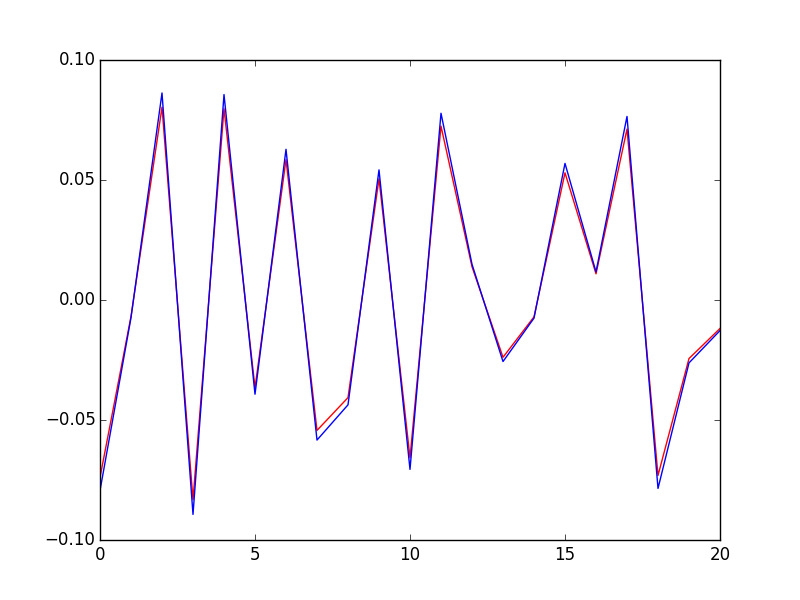
\includegraphics[height=3.25in,width=5in,angle=0]{originals.png} 
\caption{This diagram illustrates two correlated waveforms. Both waveforms are drawn i.i.d. from a Gaussian distribution, and they are correlated with covariance matrix~\usebox{\covmat}, $m=4$.}
\end{center} 
\end{figure}  

Now that we have the two waveforms, the first stage of our algorithm is to reduce the waveforms modulo the range [-1, 1]. The reduced versions of the two waveforms are shown in Figure 2. \\

\begin{figure}
\begin{center}
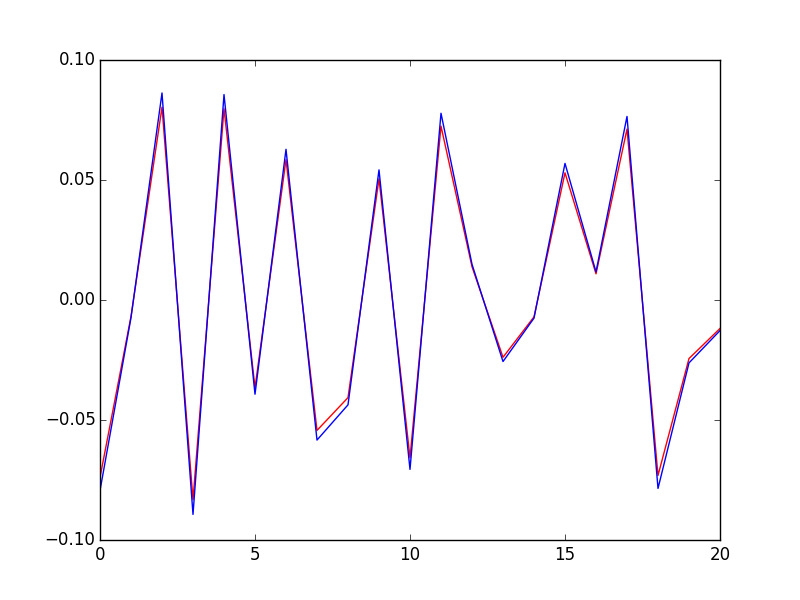
\includegraphics[height=3.25in,width=5in,angle=0]{originalsreduced.png} 
\caption{This diagram illustrates the two waveforms from Figure 1, reduced modulo the range [-1, 1].}
\end{center}
\end{figure}

Next, we quantize the two waveforms with a 4-bit quantizer. Quantizing the waveform is necessary in order to encode it digitally, because otherwise encoding it would require an arbitrarily large number of bits.\\

\begin{figure}
\begin{center}
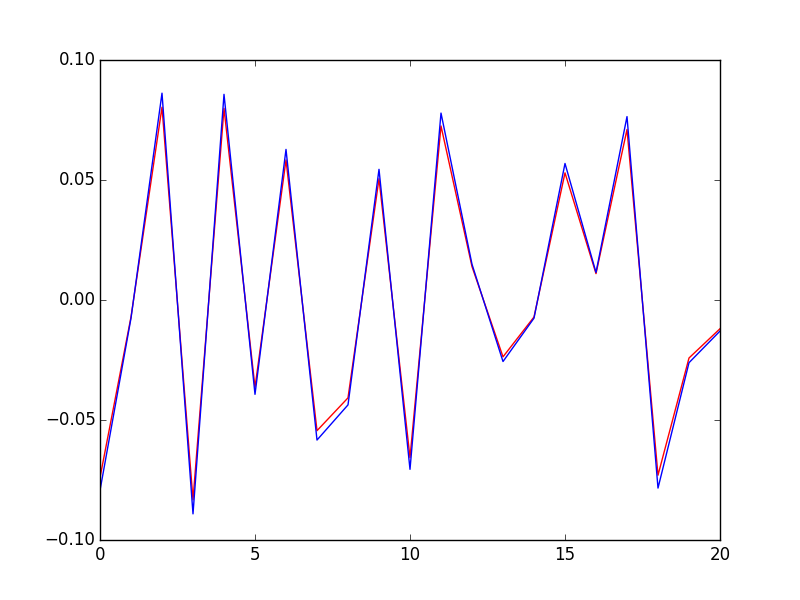
\includegraphics[height=3.25in,width=5in,angle=0]{originalquantized.png} 
\caption{The reduced versions of the two waveforms, quantized with a 4-bit quantizer. Note the similarity to Figure 2. This is our encoding of the waveform.}
\end{center}
\end{figure}

Now that we have fully encoded the waveforms, the next step is to multiply the waveforms by the matrix $A$, which has a value of~\usebox{\intmat}. This will give us a good approximation of the value of $A\vec{x}$. Figure 4 shows us the result. \\

\begin{figure}
\begin{center}
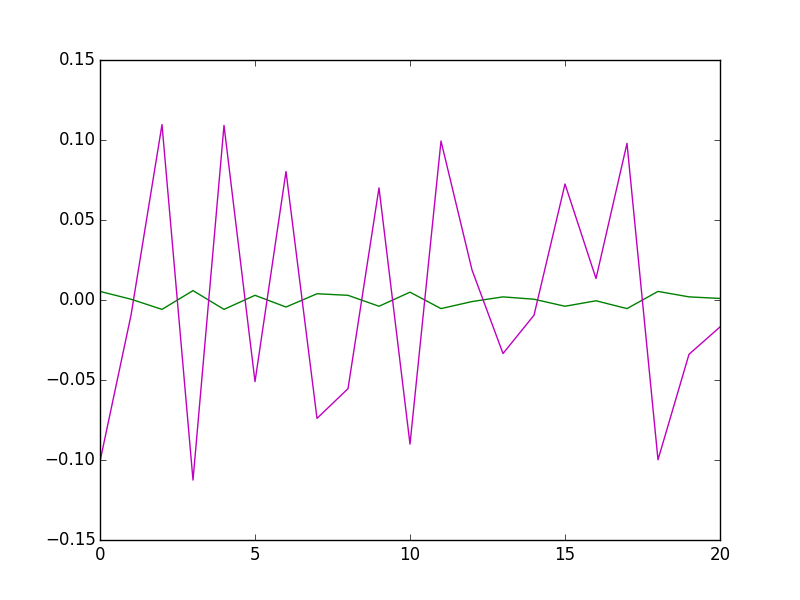
\includegraphics[height=3.25in,width=5in,angle=0]{lincombs.png} 
\caption{The reduced and quantized versions of the two waveforms (shown in Figure 3), multiplied by the matrix $A =$~\usebox{\intmat}. This will be approximately equal to $A\vec{x}$.}
\end{center}
\end{figure}

Next, we must reduce the linear combinations modulo the range [1, -1], in order to be able to multiply the result by $A^{-1}$ and retrieve our approximation of $\vec{x}$. The reduced linear combinations are shown in Figure 5. \\

\begin{figure}
\begin{center}
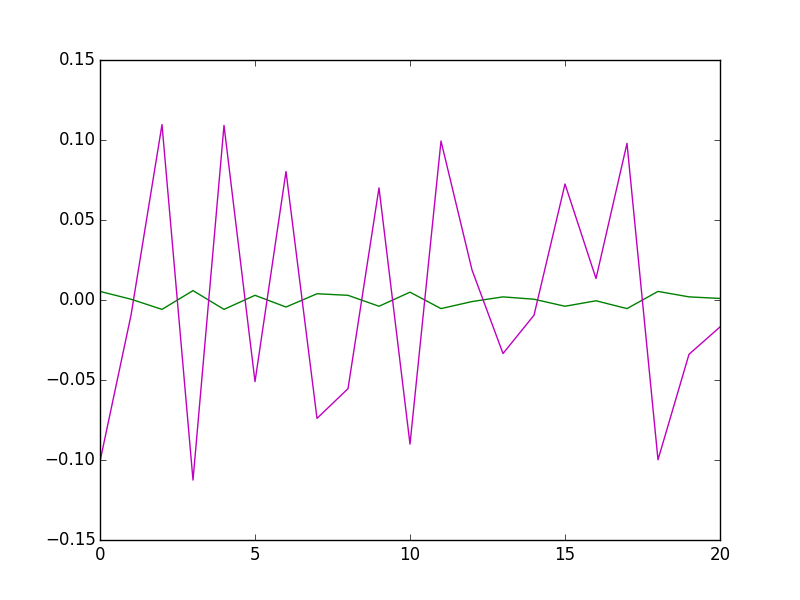
\includegraphics[height=3.25in,width=5in,angle=0]{lincombsreduced.png}
\caption{The linear combinations from Figure 4, reduced modulo the interval [-1, 1].}
\end{center}
\end{figure}

Finally, we multiply the result of the reduction shown in Figure 5 by $A^{-1}$, yielding our approximation of the original waveforms. Our approximation is shown with a thick line, whereas the original values are shown with a dotted line. \\

\begin{figure}
\begin{center}
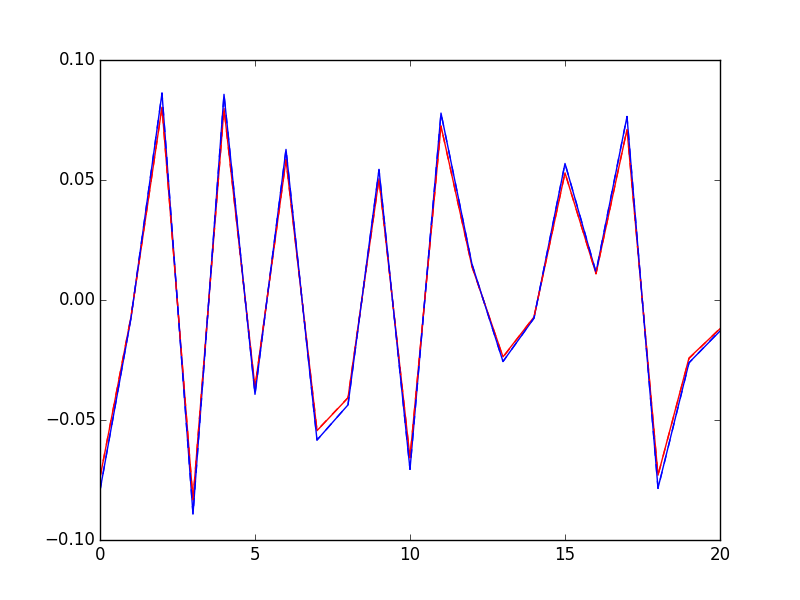
\includegraphics[height=3.25in,width=5in,angle=0]{reconstructions.png}
\caption{The final reconstructed waveforms. The original waveform is shown with a dotted line, and our approximation is shown with a thick line.}
\end{center}
\end{figure}

Figures 7 and 8 present system diagrams, for an overall summary of the encoding and decoding process, respectively. \\

%$$s \equiv (x+y) \pmod 2$$
%$$d \equiv (x-y) \pmod 2$$ \\

%Adding or subtracting the two equations together, we find:

%$$s+d \equiv 2x \pmod 2$$
%$$s-d \equiv 2y \pmod 2$$ \\

%It follows, then, that $x \equiv \frac{s+d}{2} \pmod 2$ or $x \equiv (\frac{s+d}{2} + 1) \pmod 2$. Similarly, $y \equiv \frac{s-d}{2} \pmod 2$ or $y \equiv (\frac{s-d}{2} + 1) \pmod 2$. Put more simply,

%$$x \equiv \frac{s+d}{2} \pmod 1$$
%$$y \equiv \frac{s-d}{2} \pmod 1$$ \\

%Figure 5 shows the values of $x$ and $y$ modulo 1--these are the values we can reconstruct with certainty.

%From this information, we can try to infer the true values of $x$ and $y$. Figure 6 shows the maximum a posteriori values for $x$ and $y$ given their values modulo 1 as a dotted line, superimposed on their true values as a solid line.

%\begin{figure}
%\begin{center}
%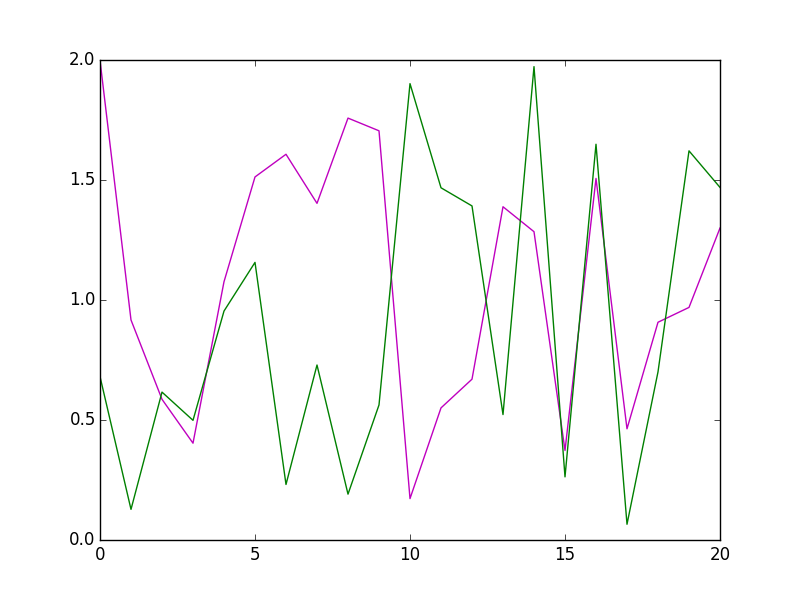
\includegraphics[height=3.25in,width=5in,angle=0]{mods.png} 
%\caption{The sum and difference waveforms, each taken modulo 2. This is our encoding of the original %values}
%\end{center}
%\end{figure}

%\begin{figure} 
%\begin{center} 
%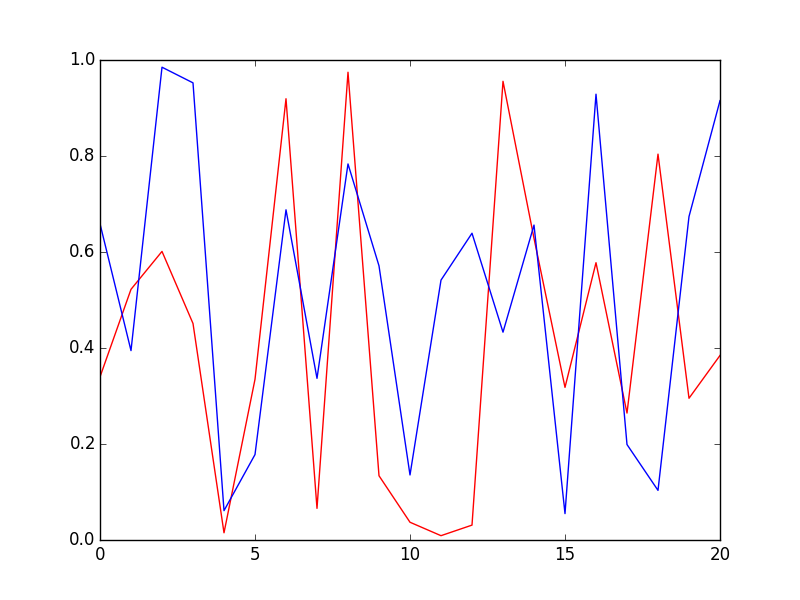
\includegraphics[height=3.25in,width=5in,angle=0]{originalmods.png} 
%\caption{The reconstructed values of $x$ and $y$ modulo 1. These values are known with certainty.}
%\end{center} 
%\end{figure}  

%\begin{figure} 
%\begin{center} 
%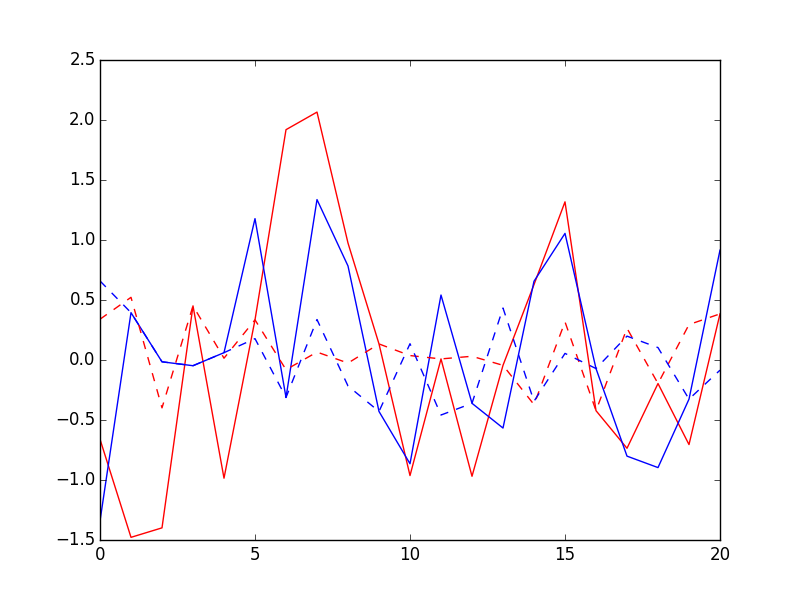
\includegraphics[height=3.25in,width=5in,angle=0]{correlatedwaveformswithguesses.png} 
%\caption{The inferred true values of $x$ and $y$, inferred using their known values modulo 1, shown as a dotted line. The solid line represents their true values.}
%\end{center} 
%\end{figure}  


%This is our general approach; in order to do this, we want to be able to perform additions and multiplications (to compute the linear combinations), followed by a modulus operation, followed by another series of additions and multiplications (solving the equations). An diagram for the encoding system overall is shown below.

\begin{figure} 
\begin{center} 
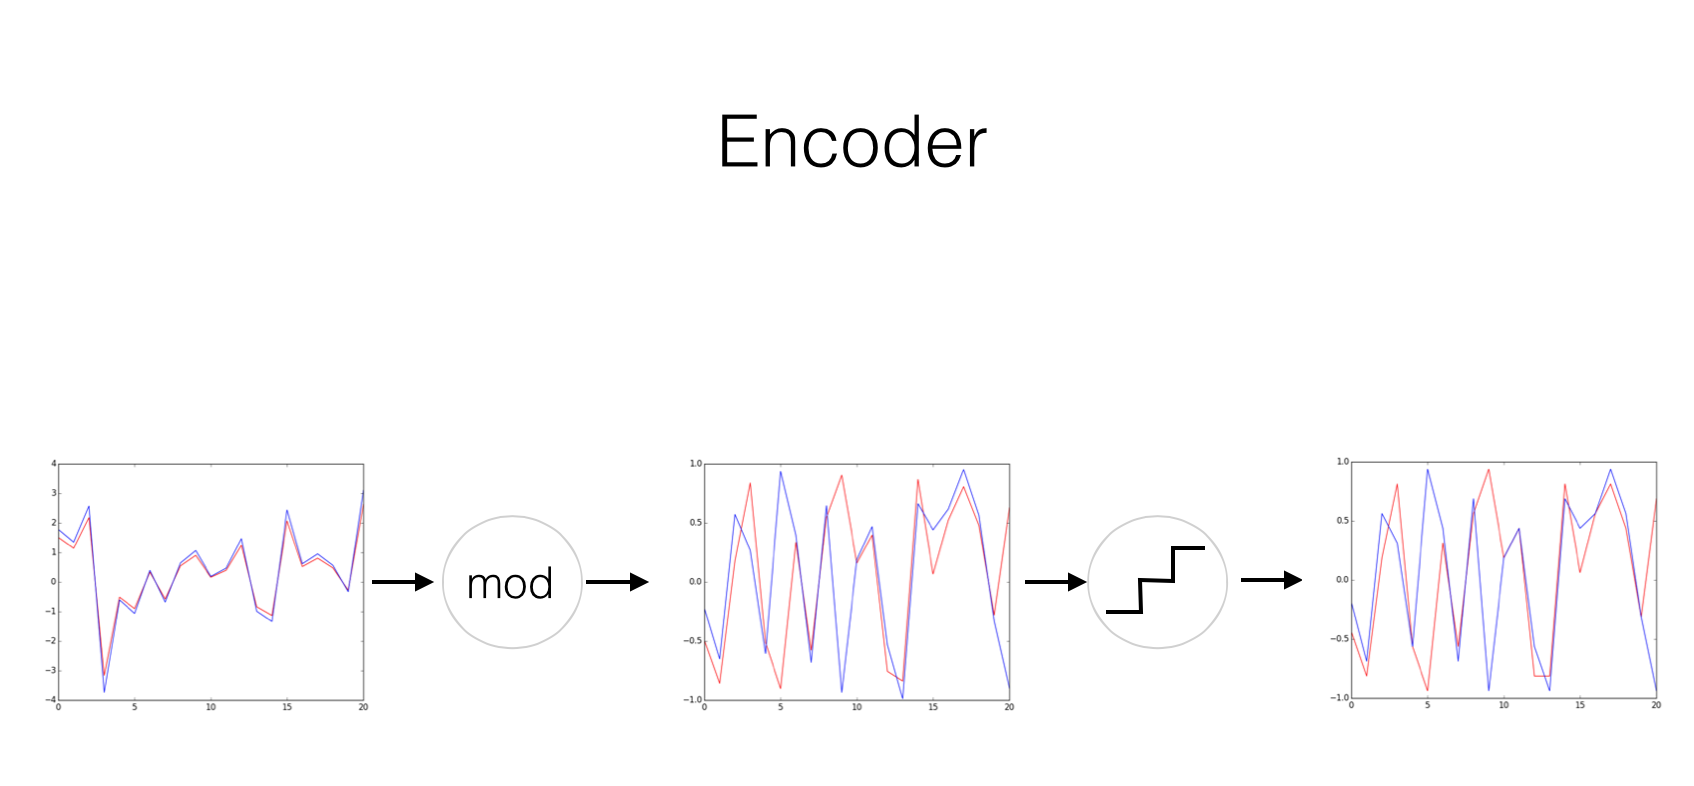
\includegraphics[scale=0.4]{encoderdiagram.png} 
\caption{A system diagram illustrating the encoding process. %, shown on the left, as linear combinations of the waveforms taken modulo some small value, shown on the right. Note that although in this example the linear combinations are $x+y$ and $x-y$ and the modulus is 2, both of these choices are parameters that could be varied.
}
\end{center}
\end{figure}

\begin{figure} 
\begin{center} 
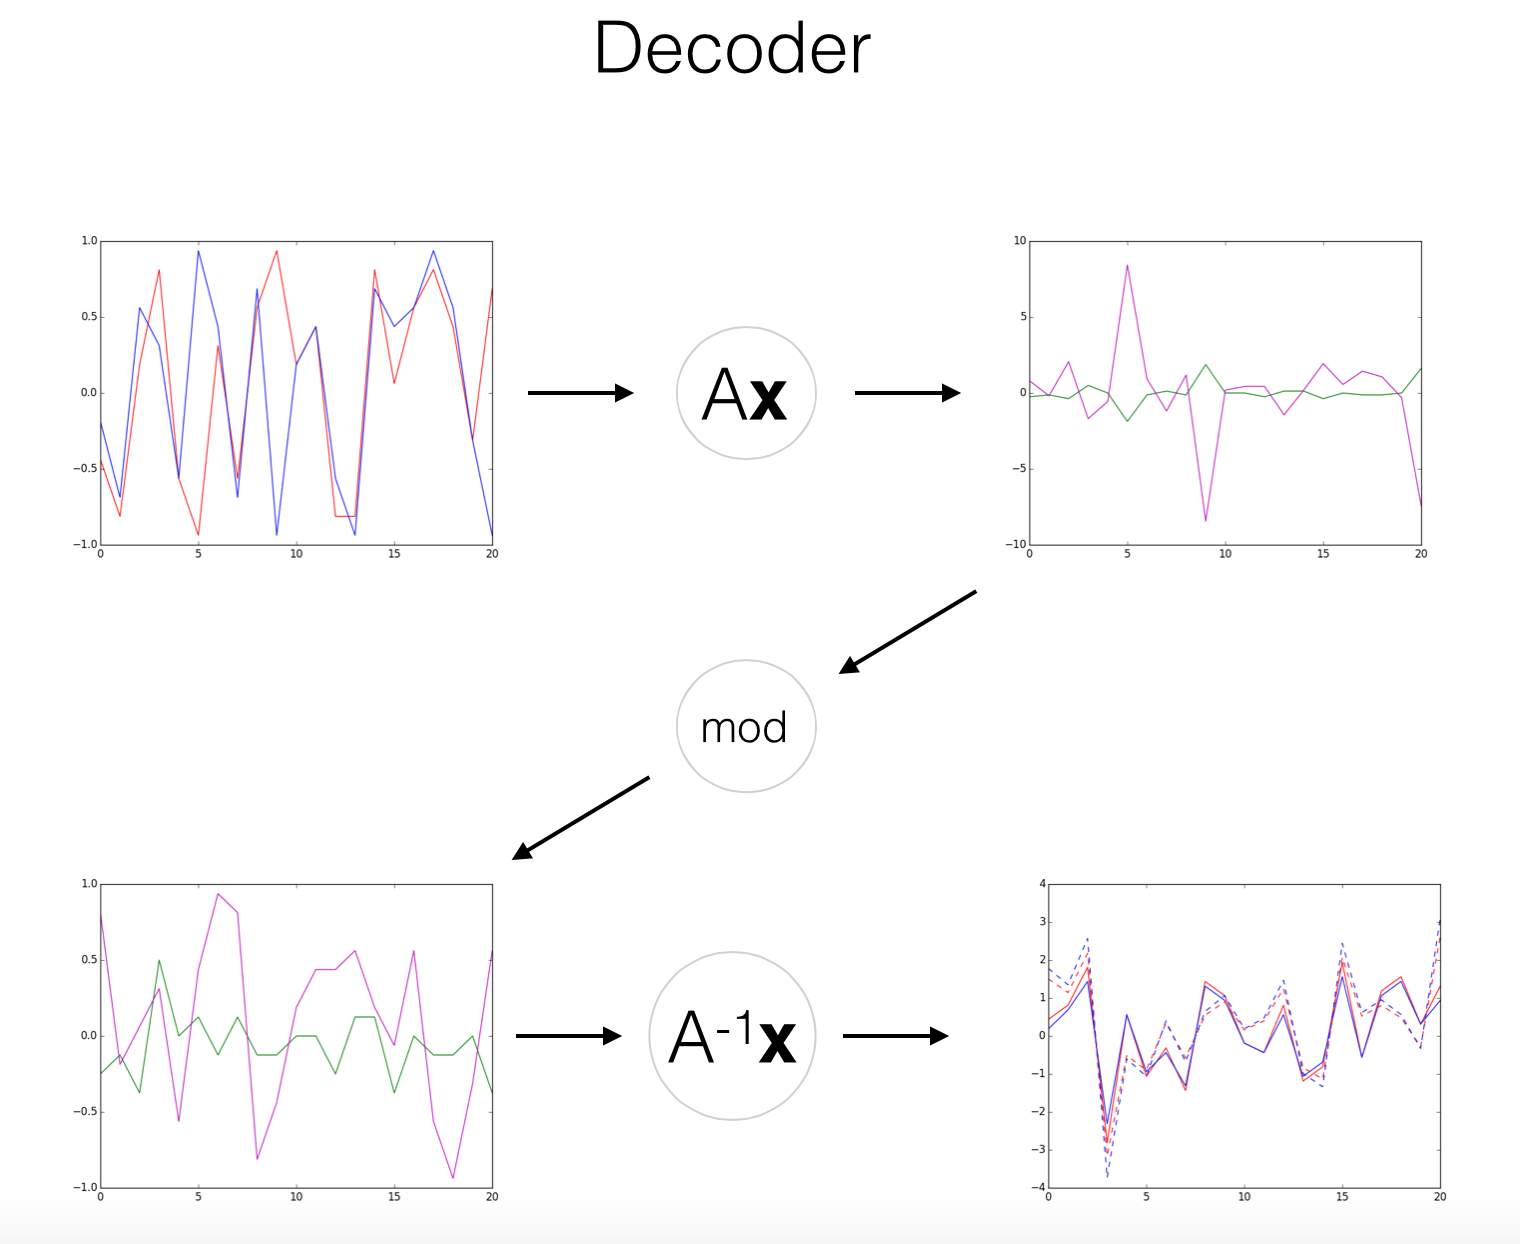
\includegraphics[scale=0.4]{decoderdiagram.png} 
\caption{A system diagram describing the decoding process. %, shown on the left, as linear combinations of the waveforms taken modulo some small value, shown on the right. Note that although in this example the linear combinations are $x+y$ and $x-y$ and the modulus is 2, both of these choices are parameters that could be varied.
}
\end{center}
\end{figure}


A variant of this method can also be applied to efficiently encode a single waveform which is not i.i.d., by taking advantage of the waveform's autocorrelation. As an example waveform of this kind, we use a waveform that's meant to represent an i.i.d. sequence of observations of a normally distributed random variable, but one that's been ``oversampled''--that is, there are many observations that are made of the waveform as it transitions from one data point to the next. Thus, each observation carries a lot of information about the next observation. \\

We simulate this effect by taking an i.i.d. sequence of observations of a normally distributed waveform, taking its Fourier transform, zeroing out the high-frequency components, and transforming back. Let $L$ denote the number of i.i.d. observations in the ``oversampled'' waveform, and let $n$ denote the number of observations we make in between the i.i.d. observations. Thus, the total number observations is $Ln$. Figure 9 shows the resulting waveform, with choices $L=32$ and $n=128$. \\

\begin{figure} 
\begin{center} 
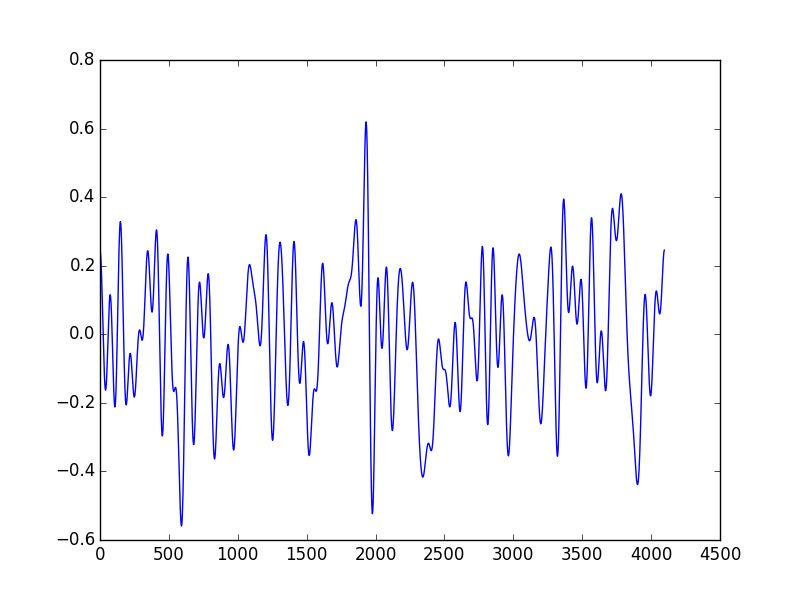
\includegraphics[scale=0.4]{oversampledwaveform.png} 
\caption{An autocorrelated waveform, with 32 i.i.d normally distributed instances and smooth extrapolation in between them.%, shown on the left, as linear combinations of the waveforms taken modulo some small value, shown on the right. Note that although in this example the linear combinations are $x+y$ and $x-y$ and the modulus is 2, both of these choices are parameters that could be varied.
}
\end{center}
\end{figure}


Naturally, we could use the approach described earlier in the paper to encode this waveform more efficiently, treating the waveform and the same waveform shifted back by one time-step as though they were two separate waveforms. This approach will work quite well! However, it won't be as good as it could be, because an autocorrelated waveform has an interesting past beyond the one time-step previous. In other words, not only the time-step before it but every time-step in the past carries useful information for predicting the next time-step. \\

In order to keep the complexity of the prediction fixed, we will fix the number of time-steps in the past that we are looking. We'll call this number $p$. \\

Each previous point carries predictive power about the next point proportional to $sinc(d)$, where $d$ is the number of the time-steps in the past the previous point was, and the $sinc$ function is defined as \\

$$sinc(x) = \sin(x)/x$$ \\

with $sinc(0) = 1$. Logically, then, an effective means of predicting the next point is to multiply each previous point by the $sinc$ of the number of time-steps ago each was, and sum the result. More precisely, we take the dot product of the $p$-dimensional vector $[sinc(1/L), sinc(2/L), \dots, sinc(p/L)]$, and the vector containing the $p$ previous points in the waveform. This procedure is the extension of the method earlier described to using many points instead of one point, of decreasing predictive value. \\

Figure 10 shows this prediction method applied to the waveform seen in Figure 9. As can be seen, the method is extremely accurate.

\begin{figure} 
\begin{center} 
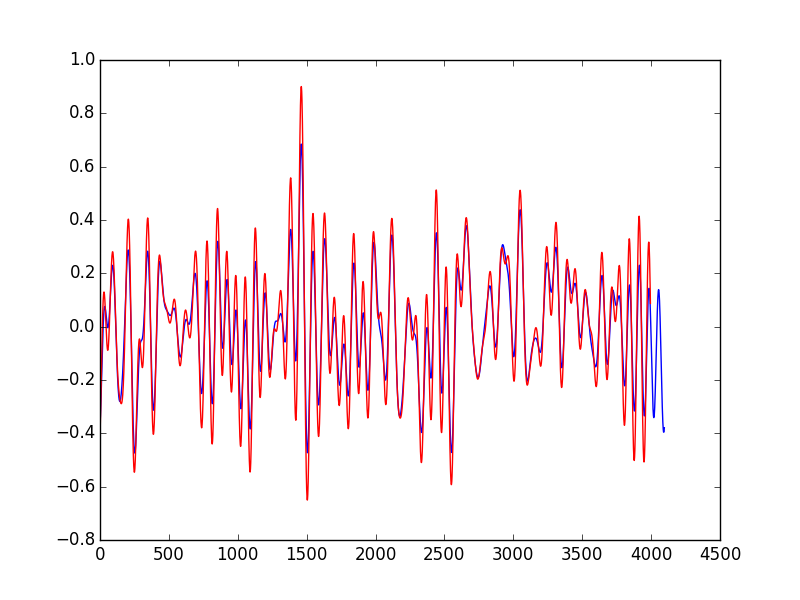
\includegraphics[scale=0.4]{oversampledwaveformwithprediction.png} 
\caption{The waveform from Figure 9, along with the prediction gained by multiplying previous points by the sinc function of how long ago they were. Red is the prediction, and blue is the true waveform.
%, shown on the left, as linear combinations of the waveforms taken modulo some small value, shown on the right. Note that although in this example the linear combinations are $x+y$ and $x-y$ and the modulus is 2, both of these choices are parameters that could be varied.
}
\end{center}
\end{figure}

\end{document}

